\documentclass[12pt]{article}
\usepackage[utf8]{inputenc}
\usepackage[english, russian]{babel}
\usepackage{graphicx, float, multicol, hyperref}

\title{Определение систематических и случайных погрешностей 
при измерении удельного сопротивления нихромовой проволоки}
\author{Балдин Виктор}

\begin{document}
    \maketitle
    
    \section{Аннотация}
    \par \textbf{Цель работы:} измерить удельное сопротивление проволоки
    и вычислить систематические и случайные погрешности при использовании
    таких измерительных приборов, как линейка, штангенциркуль, 
    микрометр, амперметр, вольтметр и мост постоянного тока. 
    \par \textbf{В работе используются:} линейка, штангенциркуль,
    микрометр, отрезок проволоки из нихрома, ампеметр 
    , вольметр, источник ЭДС, мост постоянного тока, реостат, ключ.
    \section{Теоретические сведения}
    \par Считая проволоку имеющей всюду одинаковую толщину, ее
    сопротивление можно найти по формуле: 
    \begin{equation}
        R_{\mbox{\tiny{пр}}} = \rho\frac{4l}{\pi d^2},
    \end{equation}
    где $\rho$ -- удельное сопротивление нихрома.
    
    \section{Методика измерений}
    \par \textbf{Метод 1. }Сопротивление проволоки можно найти c помощью одной из схем:
    \begin{figure}[H]
        \centering
        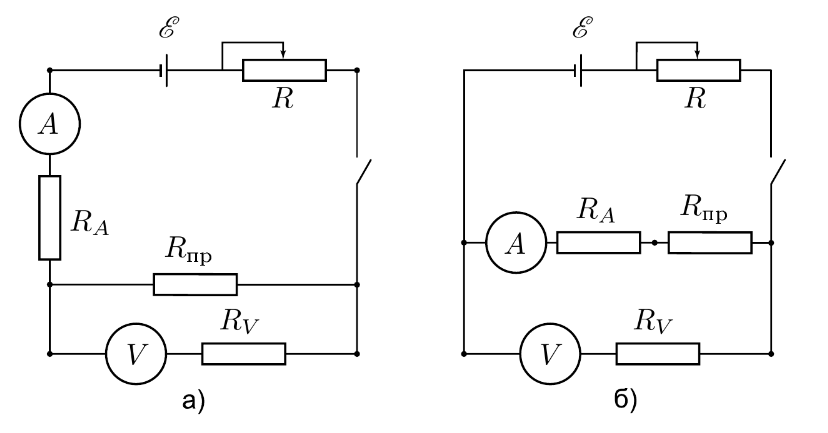
\includegraphics[scale=0.6]{circuit.png}
    \end{figure}
    Сопротивление проволоки в обоих случаях находим как
    \begin{equation}
        R_{\mbox{\tiny{пр}}} = \frac{U_V}{I_A}
    \end{equation}
    С учетом поправок, которые вносятся засчет неидеальности амперметра
    и вольтметра, реальное значение сопротивления для схемы 1:
    \begin{equation}
        R_{\mbox{\tiny{пр}}} = R_{\mbox{\tiny{пр1}}}\left(1 + 
        \frac{R_{\mbox{\tiny{пр1}}}}{R_V}\right)
    \end{equation}
    Для схемы 2:
    \begin{equation}
        R_{\mbox{\tiny{пр}}} = R_{\mbox{\tiny{пр2}}}\left(1 - 
        \frac{R_A}{R_{\mbox{\tiny{пр2}}}}\right)
    \end{equation}
    Видно, что в формуле (4) $R_A \sim R_{\mbox{\tiny{пр2}}}$,
    т. к. проволока тонкая и ее сопротивление невелико, значит, в 
    измерении может присутствовать очень существенная поправка. Поэтому
    проведем измерения на схеме 1.
    \par \textbf{Метод 2. }Поскольку и схема 1 имеет некоторую поправку, целесообразно
    потом сравнить результат с наиболее точным способом: мостом Р4833.
    
    \section{Оборудование}
    \begin{table}[H]
        \caption{Технические характеристики используемых приборов}
        \begin{tabular}{|l|c|c|}
        \hline
        \multicolumn{1}{|c|}{}   & Вольтметр           & Миллиамперметр   \\ \hline
        Система                  & Магнитоэлетрическая & Цифровая         \\ \hline
        Класс точности           & 0,5                 & 0,5              \\ \hline
        Предел измерений         & 0,3 В               & 0,15 А           \\ \hline
        Цена делений             & 5 мВ/дел            & -                \\ \hline
        Абсолюная погрешность    & 5 мВ                & 0,4 мА           \\ \hline
        Внутреннее сопротивление & 250 Ом              & 1 Ом             \\ \hline
        \end{tabular}
    \end{table}
    \textbf{Мост постоянного тока Р4833: \\}
    Класс точности: 0,1\\
    Разрадность магазина сопротивлений: 5\\
    Используемый диапазон: $10^{-4}$ -- 10 Ом (множитель $N = 10^{-2}$)\\
    Погрешность: $\pm0,01$ Ом.

    \section{Результаты измерений и обработка данных}
    \begin{enumerate}
        \item Проведем измерения диаметра проволоки в разных местах при
    помощи штангенциркуля и микрометра.
    \begin{table}[H]
        \caption{Измерение штангенциркулем}
        \begin{tabular}{|c|c|c|c|c|c|c|c|c|c|c|}
        \hline
        №                  & 1   & 2   & 3   & 4   & 5   & 6   & 7   & 8   & 9   & 10  \\ \hline
        $d$, $10^{-1}$, мм & 3,5 & 4,0 & 4,0 & 4,0 & 4,0 & 4,0 & 3,5 & 4,0 & 3,5 & 4,0 \\ \hline
        \end{tabular}
    \end{table}
    \par Случайная погрешность $\sigma_d = 0{,}3\cdot10^{-1}$ мм.
    С учетом приборной погрешности штангенциркуля и случайной среднее
    значение $d = (3{,}9\pm0{,}8)\cdot10^{-1}$ мм.
    \begin{table}[H]
        \caption{Измерение микрометром}
        \begin{tabular}{|c|c|c|c|c|c|c|c|c|c|c|}
        \hline
        №                 & 1    & 2    & 3    & 4    & 5    & 6    & 7    & 8    & 9    & 10   \\ \hline
        $d$, $10^{-2}$ мм & 35,5 & 35,5 & 35,5 & 35,0 & 35,0 & 35,0 & 35,0 & 35,5 & 35,0 & 35,5 \\ \hline
        \end{tabular}
    \end{table}
    С учетом случайной $\sigma_d = 0,3\cdot10^{-2}$ мм и приборной $\delta_d = 0,5\cdot10^{-2}$ мм 
     погрешности $d = (35{,}3\pm0{,}8)\cdot
    10^{-2}$ мм. Будем использовать это значение, т. к. оно более точное.
    \item Перейдем к измерению сопротивления. На схеме 1 будем регулировать
    сопротивление реостата, чтобы изменять силу тока и напряжение на
    проволоке. Снимем зависимость:
    \begin{table}[H]
        \caption{ВАХ проволоки}
        \begin{tabular}{|cc|cc|cc|}
        \hline
        \multicolumn{2}{|c|}{$l = 20$ см}       & \multicolumn{2}{c|}{$l = 30$ см}       & \multicolumn{2}{c|}{$l = 50$ см}       \\ \hline
        \multicolumn{1}{|c|}{$U$, мВ} & $I$, мА & \multicolumn{1}{c|}{$U$, мВ} & $I$, мА & \multicolumn{1}{c|}{$U$, мВ} & $I$, мА \\ \hline
        \multicolumn{1}{|c|}{740}     & 350,0   & \multicolumn{1}{c|}{720}     & 235,4   & \multicolumn{1}{c|}{720}     & 143,0   \\ \hline
        \multicolumn{1}{|c|}{650}     & 309,3   & \multicolumn{1}{c|}{670}     & 219,8   & \multicolumn{1}{c|}{610}     & 120,8   \\ \hline
        \multicolumn{1}{|c|}{545}     & 259,6   & \multicolumn{1}{c|}{540}     & 175,9   & \multicolumn{1}{c|}{512}     & 102,4   \\ \hline
        \multicolumn{1}{|c|}{455}     & 217,1   & \multicolumn{1}{c|}{475}     & 154,4   & \multicolumn{1}{c|}{390}     & 77,9    \\ \hline
        \multicolumn{1}{|c|}{375}     & 179,9   & \multicolumn{1}{c|}{365}     & 119,7   & \multicolumn{1}{c|}{290}     & 57,9    \\ \hline
        \multicolumn{1}{|c|}{330}     & 157,4   & \multicolumn{1}{c|}{250}     & 82,6    & \multicolumn{1}{c|}{130}     & 26,0    \\ \hline
        \multicolumn{1}{|c|}{265}     & 126,1   & \multicolumn{1}{c|}{165}     & 52,4    & \multicolumn{1}{c|}{45}      & 9,9     \\ \hline
        \multicolumn{1}{|c|}{190}     & 89,8    & \multicolumn{1}{c|}{60}      & 27,3    & \multicolumn{1}{c|}{}        &         \\ \hline
        \multicolumn{1}{|c|}{130}     & 60,8    & \multicolumn{1}{c|}{}        &         & \multicolumn{1}{c|}{}        &         \\ \hline
        \multicolumn{1}{|c|}{100}     & 48,4    & \multicolumn{1}{c|}{}        &         & \multicolumn{1}{c|}{}        &         \\ \hline
        \multicolumn{1}{|c|}{40}      & 10,1    & \multicolumn{1}{c|}{}        &         & \multicolumn{1}{c|}{}        &         \\ \hline
        \end{tabular}
        \end{table}
    Для каждой длины построим графики $I(U)$ (см. приложение).
    \item При помощи метода наименьших квадратов найдем $R_{\mbox{\tiny{ср}}}$:
    \[
        R_{\mbox{\tiny{ср}}} = \frac{\sum_{i = 1}^{n} U_iI_i}
        {\sum_{i = 1}^{n} I_i^2} 
    \]
    Случайную погрешность $R_{\mbox{\tiny{ср}}}$ при этом можно определить как
    \[
        \sigma_R^{\mbox{\tiny{сл}}} = \frac{1}{\sqrt{n}}\sqrt{\frac{\langle U^2\rangle}{\langle I^2\rangle} - R_{\mbox{\tiny{ср}}}^2}    
    \]
    Систематическую погрешность считаем по формуле:
    \[
        \sigma_R^{\mbox{\tiny{сист}}} = R_{\mbox{\tiny{ср}}}\sqrt{\left(\frac{
        \sigma_U}{U}\right)^2 + \left(\frac{\sigma_I}{I}\right)^2},
    \] где $U = 740$ мВ, $I = 250$ мА.
    \item Проведем измерения сопротивлений на мосте постоянного тока Р4833
    результат занесем в таблицу 5, в силу малости его погрешности считаем, что
    по формуле (1)
    \[
        \frac{\sigma_{\rho}}{\rho} \approx 2\frac{2\sigma_d}{d}
    \]
    \item Занесем в таблицу посчитанные таким образом значения, а также рассчитаем
    $R_{\mbox{\tiny{пр}}}$ по формуле (3), взяв внутреннее сопротивление
    вольметра равным $R_V = 250$ Ом:
    \begin{table}[H]
        \caption{Сопротивления}
        \begin{tabular}{|c|c|c|c|c|c|c|}
        \hline
        $l$, см & $R_{\mbox{\tiny{ср}}}$, Ом & $\sigma_R^{\mbox{\tiny{сл}}}$, Ом & $\sigma_R^{\mbox{\tiny{сист}}}$, Ом & $R_{\mbox{\tiny{пр}}}$, Ом & $\sigma_R$, Ом & $R_{\mbox{\tiny{мост}}}$, Ом \\ \hline
        20      & 2,08                       & 0,04                              & 0,01                                & 2,10                        & 0,05           & 2,148                       \\ \hline
        30      & 3,13                       & 0,06                              & 0,02                                & 3,17                       & 0,08           & 3,129                       \\ \hline
        50      & 5,00                          & 0,15                              & 0,03                                & 5,10                        & 0,18           & 5,158                       \\ \hline
        \end{tabular}
    \end{table}
    Поправка $R_{\mbox{\tiny{ср}}}/R_V \ll 1$, поэтому ее погрешность можно не учитывать.
    \item Согласно формуле (1) зависимость $R_{\mbox{\tiny{пр}}}(l)$ должна быть линейной, поэтому
    применим МНК для анализа данных, представленных в таблице 5. Погрешность найдем как
    \[
        \frac{\sigma_{\rho}}{\rho} = \sqrt{\left(\frac{\sigma_R}{R}\right)^2 +
        \left(\frac{2\sigma_d}{d}\right)^2}
    \]
    \item Результаты вычисления удельного сопротивления и его погрешности для использованных методов в таблице:
    \begin{table}[H]
        \caption{Результаты}
        \begin{tabular}{|c|c|c|}
        \hline
                                    & Схема         & Мост          \\ \hline
        $\rho$, $10^{-6}$ Ом$\cdot$м & $0,95\pm0,06$ & $0,95\pm0,03$ \\ \hline
        \end{tabular}
    \end{table}
    \end{enumerate}
    
    \section{Анализ результатов и вывод}
    \par По итогам работы было получено значение удельного сопротивления нихрома, близкое к табличному, которое лежит в
    диапазоне 1,05 ... $1,40\cdot10^{-6}$ Ом$\cdot$м (источник: 
    \url{https://ru.wikipedia.org/wiki/%D0%9D%D0%B8%D1%85%D1%80%D0%BE%D0%BC#:~:text=
    %D0%A3%D0%B4%D0%B5%D0%BB%D1%8C%D0%BD%D0%BE%D0%B5%20%D1%81%D0%BE%D0%BF%D1%80%D0%BE
    %D1%82%D0%B8%D0%B2%D0%BB%D0%B5%D0%BD%D0%B8%D0%B5%201%2C13%20%D0%9E%D0%BC,%D1%82%D0
    %B5%D0%BC%D0%BF%D0%B5%D1%80%D0%B0%D1%82%D1%83%D1%80%D0%B0%20%D0%BF%D0%BB%D0%B0%D0
    %B2%D0%BB%D0%B5%D0%BD%D0%B8%D1%8F%201400%20%C2%B0C.}).
    \par Измерение на Р4833 позволило сократить погрешность примерно в 2 раза, из чего можно заключить, что
    мостиковые схемы лучше всего подходят для точного измерения сопротивлений.
    \par Поскольку оба метода дали значение ниже типичного для нихрома, также можно предположить, что перед нами
    был сплав c некоторыми примесями. Другая возможная причина состоит в том, что нам не удалось подтвердить
    однородность проволоки по диаметру в достаточной степени ($\sigma_d^2 \sim \delta_d^2$).

\end{document}
